\documentclass[10pt,a4paper,twoside]{article}
\usepackage{latexsym}      % needed math symbols
\usepackage{hyperref}
\hypersetup{
 colorlinks=true,
 citecolor=blue,
 linkcolor=blue,
 urlcolor=blue,
 pdfpagemode=UseNone,
 pdfstartview=FitH}
\usepackage{graphicx}      % for importing eps figures
\usepackage{amsmath}       % for advanced math symbols
\usepackage[affil-sl]{authblk} 			% found in preprint bundle package, http://ctan.org/pkg/preprint
\usepackage[margin=2.5cm]{geometry} % paper and margin formats as set by SPP
\usepackage{subfig}

\parindent 0.5cm    % paragraphs indent
\topmargin=-2cm

% SPP details
\newcommand{\spp}{38\textsuperscript{th}}
\newcommand{\sppvenue}{Legazpi City, Albay}
\newcommand{\sppdate}{3--6 June 2020}


% title style
\newcommand*{\TitleFont}{\bfseries \Large }

% authblk style
\newcommand{\authorsep}{,\negmedspace}
\newcommand{\lastauthorsep}{}
\makeatletter
\renewcommand\AB@authnote[1]{{\textsuperscript{\normalfont#1}\ }}
\renewcommand\Authsep{}
\renewcommand\Authands{and }
\renewcommand\Authfont{\small {\bfseries}}
\renewcommand\Affilfont{\small	\itshape}
\setlength{\affilsep}{5pt}
\makeatother
\newcommand{\corremail}{\rm Corresponding author:~}

% remove date
\date{}

% for abstract style
\makeatletter
\newbox\abstract@box
\renewenvironment{abstract}
   {\global\setbox\abstract@box=\vbox\bgroup
     \hsize=\textwidth\linewidth=\textwidth
    \vspace{-2em}
		\small
		%\begin{center}
		{\hspace{1.2em}\bfseries \abstractname\vspace{.0em}\vspace{\z@} }%
		%\end{center}
    \quotation}
  {\endquotation\egroup}
\expandafter\def\expandafter\@maketitle\expandafter{\@maketitle
	\ifvoid\abstract@box\else\unvbox\abstract@box\if@twocolumn\vskip1.5em\fi\fi}
\makeatother
\providecommand{\keywords}[1]{\vspace{.5em}\noindent \mdseries{{Keywords:}} #1}
\providecommand{\DOI}[1]{\vspace{#1\baselineskip}}
\providecommand{\dateline}[1]{\vspace*{-1\baselineskip}\normalsize Submitted: #1\vspace*{-1.5\baselineskip}}

% for section formatting style
\makeatletter
\renewcommand\section{\@startsection
   {section}{1}{0pt}%
   {-\baselineskip}%
   {0.1\baselineskip}%
   {\normalfont\large\bfseries}}%
\renewcommand\subsection{\@startsection
   {subsection}{1}{0pt}%
   {-\baselineskip}%
   {0.1\baselineskip}%
   {\normalfont\bfseries}}%
\makeatother
\renewcommand\thesection{\arabic{section}}

% for the figure and tables, captions
\usepackage{booktabs}
\usepackage{dcolumn}
\newcolumntype{d}[1]{D{.}{.}{#1}}

\usepackage{caption}
\captionsetup[table]{position=above,font={rm,small}}
\captionsetup[figure]{font={rm,small}}

% for citations formatting style
\usepackage[numbers,square,sort&compress]{natbib}
\setlength\bibsep{1pt}

%%for first page styling 
\providecommand{\articlenum}[0]{}
\usepackage{fancyhdr}
\fancypagestyle{titlestyle}
{
\renewcommand{\headrulewidth}{0pt}
\renewcommand{\footrulewidth}{0.1pt}
\fancyhf[l]{}
\fancyhf[c]{ }
\fancyhf[r]{ }
\fancyfoot[l]{}
\fancyfoot[c]{\href{https://paperview.spp-online.org/proceedings/issue/archive}{Proceedings of the Samahang Pisika ng Pilipinas} \\ \href{https://paperview.spp-online.org/proceedings/issue/view/SPP-2020}{\spp\,Samahang Pisika ng Pilipinas Physics Conference}\\ \sppvenue, \sppdate \\ \articlenum 1}
\fancyfoot[r]{}
}

% styling for the second page onwards
\renewcommand{\headrulewidth}{0pt}
\renewcommand{\footrulewidth}{0.1pt}
\fancyhf[l]{}
\fancyhf[r]{}
\fancyhf[c]{}
\fancyfoot[l]{}
\fancyfoot[c]{\href{https://paperview.spp-online.org/proceedings/issue/archive}{Proceedings of the Samahang Pisika ng Pilipinas}  \\ \href{https://paperview.spp-online.org/proceedings/issue/view/SPP-2020}{\spp\,Samahang Pisika ng Pilipinas Physics Conference}\\ \sppvenue, \sppdate \\ \articlenum \thepage}
\fancyfoot[r]{}
\pagestyle{fancy}

% other packages and macros
\usepackage{bm}
\renewcommand{\vec}[1]{\text{\bfseries #1}}

\usepackage{physics}
\usepackage{amsfonts}
\usepackage{graphicx}
\graphicspath{{images/}}

%  Editorial staff will uncomment the next line
% \providecommand{\artnum}[0]{XX-XX}
% \renewcommand{\articlenum}[0]{SPP-\the\year-\artnum-}

\begin{document}

\title{\TitleFont Characterization of reconstruction error in compressively sampled speech}

\author[*\negthickspace]{Kenneth V.~Domingo}
\author[ ]{Maricor N.~Soriano
\lastauthorsep}
\affil[ ]{National Institute of Physics, University of the Philippines, Diliman, Quezon City, Philippines}
\affil[*]{\corremail{kdomingo@nip.upd.edu.ph} }


\begin{abstract}
\noindent
Modern signal acquisition technologies are made possible by the Nyquist-Shannon sampling theorem (NST). However, this paradigm is extremely wasteful as the signal is compressed before storing it by systematically discarding the imperceptible information. Compressive sensing (CS) aims to directly sense the information that would otherwise survive this compression stage. Current literature focus exclusively on either audio or image signals, as well as quantifying their reconstruction quality with ambiguous metrics. In this paper, we compressively sample signals of arbitrary dimensions such as those consisting of combinations of audio and images, as well as quantify the reconstruction quality using metrics that are perceptually intuitive.

\keywords{compressive sensing, signal processing, compressive speech enhancement}

\end{abstract}

\maketitle
\thispagestyle{titlestyle}

\section{Introduction}\label{sec:intro}
Conventional sensing devices are based on the Nyquist-Shannon sampling theorem (NST), which states that given a signal's bandwidth, one can capture all the pertinent information about that signal if it is sampled at a rate

\begin{equation} \label{eq:nst}
	f_S \geq 2f_B
\end{equation}

\noindent where $f_B$ is the signal's highest frequency component, and $2f_B$ is known as the Nyquist rate \cite{Shannon1949}. After this sampling process, the information is compressed by exploiting the signal's natural compressibility in some domain. For regular consumer-grade and even commercial-grade applications, this tried-and-true method of sampling and systematically discarding the imperceptible information works flawlessly. However, in certain situations when transmission bandwidth and/or storage comes at a premium, this process is highly wasteful \cite{Candes2008b}. Cand\'{e}s et al. \cite{Candes2006} and Donoho et al. \cite{Donoho2006} independently pioneered compressive sensing (CS), which could directly sample the portions of a signal that would otherwise survive the compression stage in conventional sampling. In this new sampling paradigm, we consider the linear model of signal acquisition

\begin{equation}\label{eq:cesa}
	\vec{y} = \vec{A}\vec{x} \equiv \innerproduct{\vec{x}}{\vec{a}_k}
\end{equation}

In other words, the signal vector $\vec{x} \in \mathbb{R}^n$ is correlated with the basis waveforms $\vec{a}_k$ to yield a compressed information vector $\vec{y} \in \mathbb{R}^m$, where $m \ll n$. This causes the task of recovering $\vec{x}$ from $\vec{y}$ impossible since there exist an infinite number of candidate solutions $\bm\hat{\vec{x}}$ which satisfy \eqref{eq:cesa}. This can be circumvented by enforcing constraints based on models of natural signals, as well as those based on optimization techniques. In particular, reconstruction can be achieved by enforcing sparsity and incoherence constraints \cite{Candes2008b}. From this, the process of reconstruction is then recast into a general minimization problem

\begin{equation}\label{eq:minl1}
	\min_{\vec{x}} \norm{\vec{x}}_1 \quad \textrm{subject to} \quad \vec{A}\vec{x} = \vec{y}
\end{equation}

\noindent where $\norm{\vec{x}}_1$ denotes the $\ell_1$ norm of $\vec{x}$.


\section{Methodology}

\section{Results and Discussion}

\begin{figure}[tb]
	\centering
	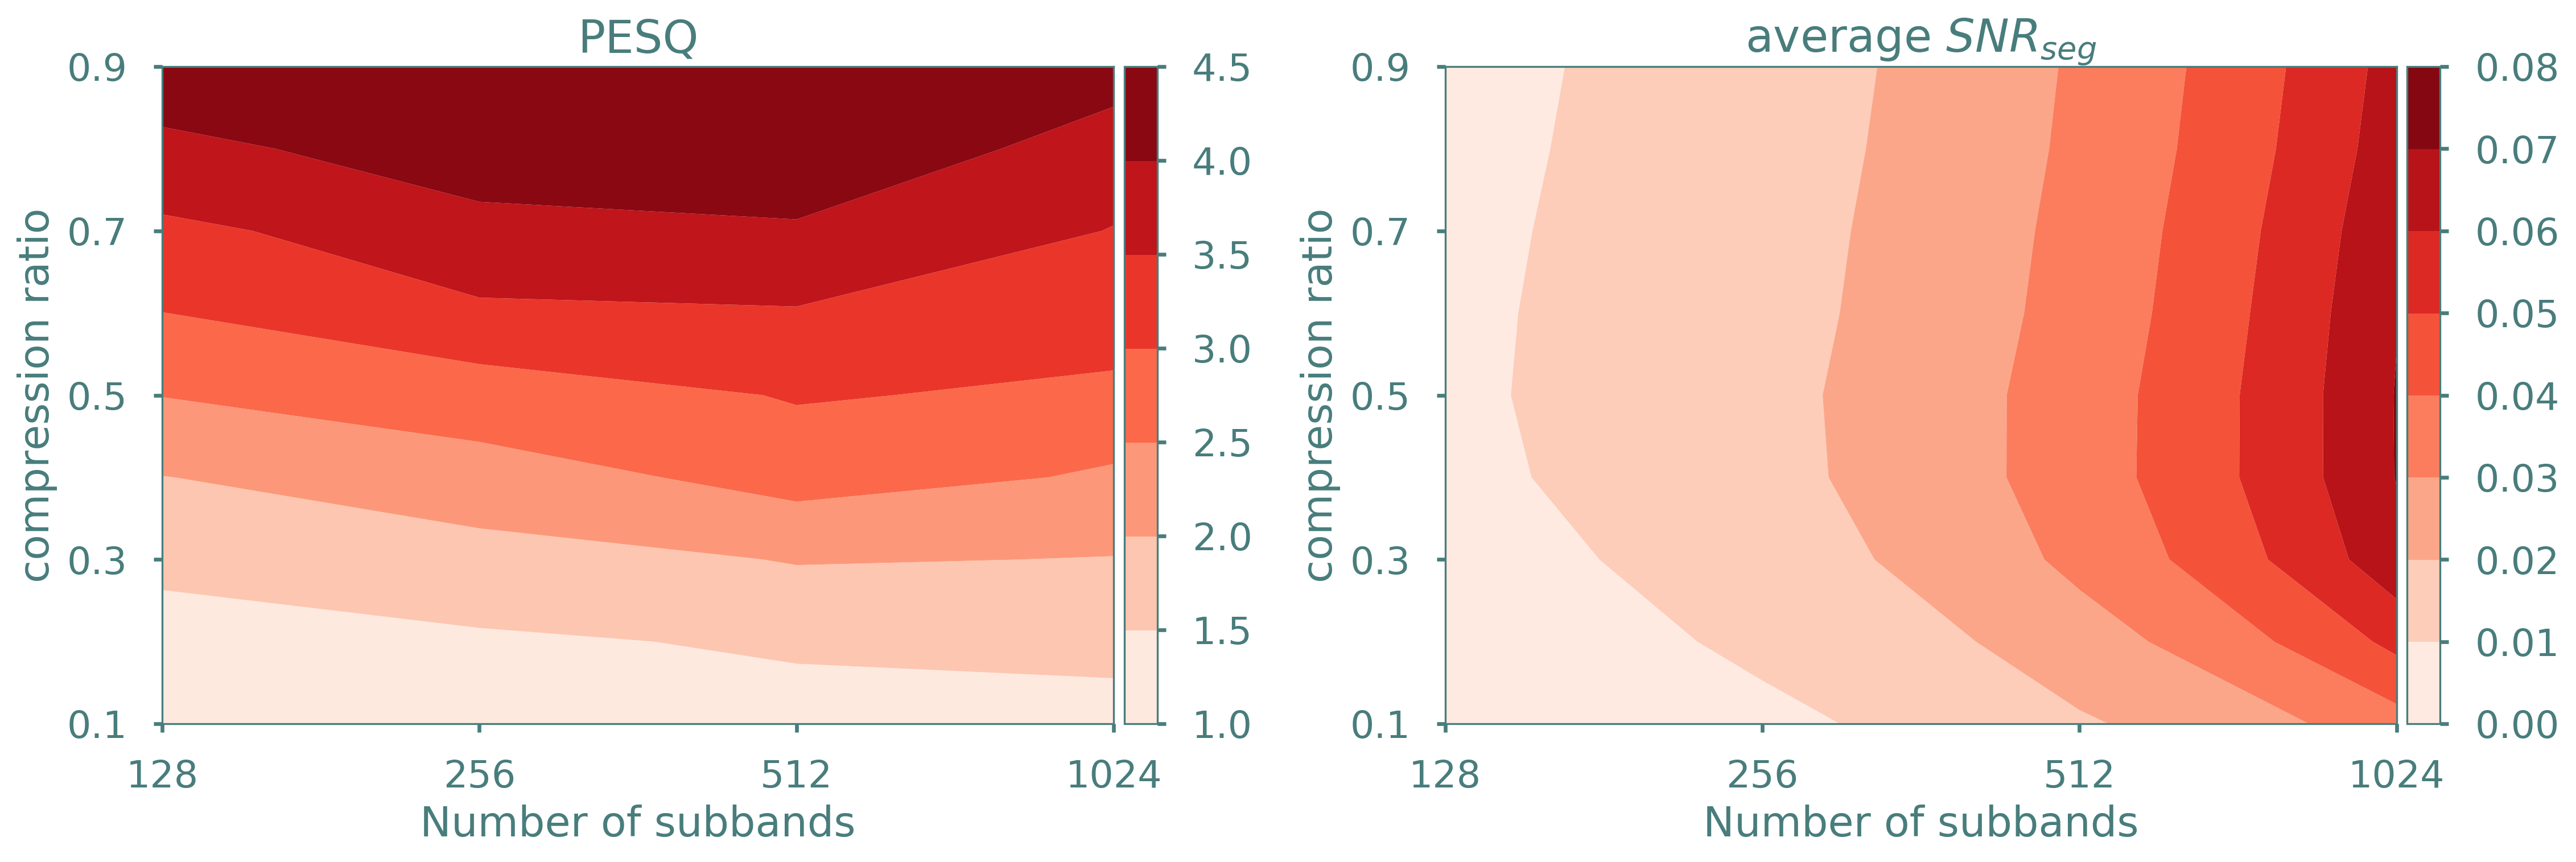
\includegraphics[width=\textwidth]{clean-pesq-snr.png}
	\caption{Two most commonly used metrics in evaluating quality of reconstructed speech recordings. PESQ is sensitive to the signal compression (left), while the average segmental SNR is sensitive to the number of subbands (right).}
	\label{fig:pesq-snr}
\end{figure}


\section{Conclusions}
Here is the Summary or Conclusions section.


\bibliographystyle{spp-bst}
\bibliography{bibfile}

\end{document}